\section{Desarrollo Experimental 3}

Para este experimento montaremos el siguiente circuito usando solamente dos multimetros, uno true RMS y otro de Vmedio.

\begin{figure}[H]
    \centering
    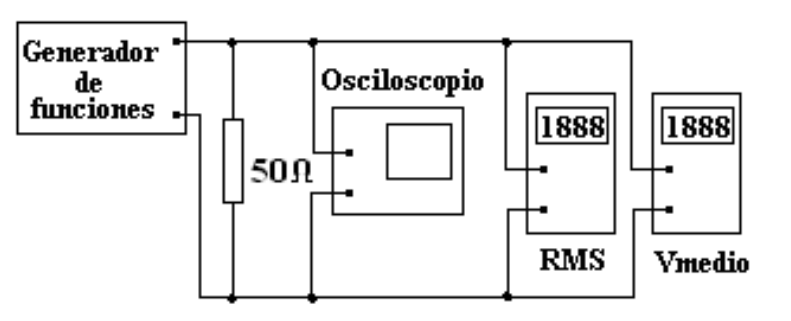
\includegraphics[width=0.5\textwidth]{images/esquema3.png}
    \caption{Conexiones realizadas}
    \label{fig:conexiones3}
\end{figure}

Seleccionamos los rangos de los instrumentos y completamos la siguiente tabla:

\begin{table}[H]
\resizebox{\columnwidth}{!}{%
\begin{tabular}{c|cc|c}
\cline{2-3}
\multicolumn{1}{l|}{}                                                                   & \multicolumn{2}{l|}{Rango: 4V C.A.} & \multicolumn{1}{l}{}         \\ \hline
\multicolumn{1}{|c|}{Generador} &
  \multicolumn{1}{c|}{\begin{tabular}[c]{@{}c@{}}RMS\\ lectura\end{tabular}} &
  \begin{tabular}[c]{@{}c@{}}Vmedio\\ lectura\end{tabular} &
  \multicolumn{1}{c|}{$e\%$} \\ \hline
\multicolumn{1}{|c|}{\begin{tabular}[c]{@{}c@{}}50Hz\\ 5Vpap\\ Cuadrada\end{tabular}}   & \multicolumn{1}{c|}{2.521}  & 2.75  & \multicolumn{1}{c|}{9.56\%}  \\ \hline
\multicolumn{1}{|c|}{\begin{tabular}[c]{@{}c@{}}50Hz\\ 5Vpap\\ Triangular\end{tabular}} & \multicolumn{1}{c|}{1.418}  & 1.3   & \multicolumn{1}{c|}{-7.62\%} \\ \hline
\end{tabular}%
}
\end{table}

\section{Desarrollo Experimental 4}

En este experimento mediremos la forma de onda proveniente de un circuito con control de ángulo de conducción, para ello haremos uso de un circuito controlador de angulo de conducción del tipo que se emplea como regulador de brillo en lámparas incandescentes (Dimmer). 

\begin{figure}[H]
    \centering
    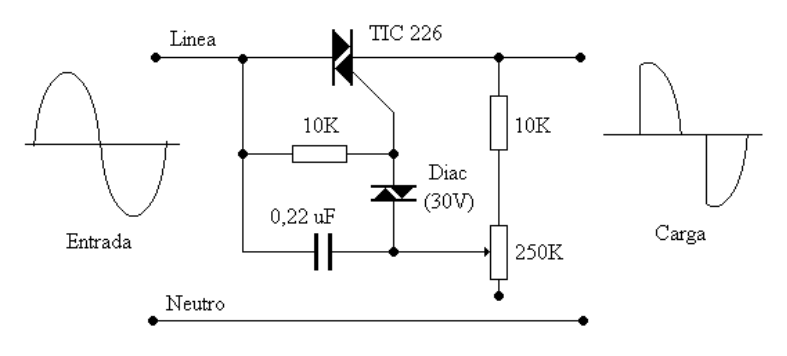
\includegraphics[width=0.5\textwidth]{images/esquema4.png}
    \caption{Conexiones realizadas}
    \label{fig:conexiones4}
\end{figure}

Para mayor seguridad usaremos un transformador de aislamiento de línea para protejer el osciloscopio.\\
La conexión a realizar es la siguiente: 

\begin{figure}[H]
    \centering
    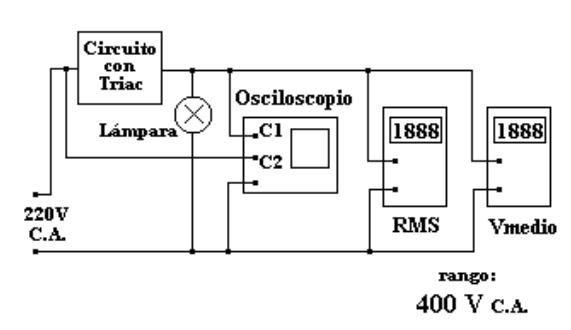
\includegraphics[width=0.5\textwidth]{images/esquema4a.png}
    \caption{Conexiones realizadas}
    \label{fig:conexiones4a}
\end{figure}

Ajustamos el osciloscopio en 5V/div y XXms/div, ademas de tener previamente la punta en x10.\\

Ahora mediremos el valor de tensión de entrada

\begin{equation*}
    V_{in} = 234.5V
\end{equation*}

Y luego variaremos el control del ángulo de conduccion del circuito con Triac. Obtendremos la mayor candidad de lecturas posibles para tensiones de salida con cada instrumento, mientras verificamos el angulo de conduccion con el osciloscopio.\\

Luego de obtener las lecturas, completamos la siguiente tabla:

\begin{table}[H]
\resizebox{\columnwidth}{!}{%
\begin{tabular}{|c|c|c|c|c|c|c|}
\hline
\multicolumn{1}{|l|}{fase} &
  \begin{tabular}[c]{@{}c@{}}Vo(1)\\ Volts\end{tabular} &
  \begin{tabular}[c]{@{}c@{}}Vo(2)\\ Volts\end{tabular} &
  \begin{tabular}[c]{@{}c@{}}Vo/Vi\\ (1)\end{tabular} &
  \begin{tabular}[c]{@{}c@{}}Vo/Vi\\ (2)\end{tabular} &
  \begin{tabular}[c]{@{}c@{}}Incertidumbre\\ medición 1\end{tabular} &
  \begin{tabular}[c]{@{}c@{}}Incertidumbre\\ medición 2\end{tabular} \\ \hline
0      & 0     & 0   & 0    & 0    & AAAA  & BBBB \\ \hline
30     & 40    & 14  & 0.17 & 0.06 & CCCC  & DDDD \\ \hline
60     & 112.7 & 60  & 0.48 & 0.25 & EEEE  & FFFF \\ \hline
90     & 173.3 & 121 & 0.74 & 0.51 & GGGG  & HHHH \\ \hline
120    & 208   & 170 & 0.88 & 0.72 & IIIII & JJJJ \\ \hline
148.32 & 228.3 & 211 & 0.97 & 0.9  & KKKK  & LLLL \\ \hline
\end{tabular}%
}
\end{table}
